% New commands
\newcommand{\Zfull}{[\mathcal Z^{(1)} + 2\mathcal Z^{(2)}]}
\newcommand{\Zone}{\mathcal Z^{(1)}}
\newcommand{\Ztwo}{\mathcal Z^{(2)}}
\newcommand{\Zi}{\mathcal Z^{(i)}}

\newcommand{\B}{\mathcal B}
\newcommand{\Set}{Set}
\newcommand{\HB}{H\mathcal B}
\newcommand{\HSet}{HSet}
\newcommand{\E}{\mathbf E}
\newcommand{\Species}{Species}
%-------------------------------------------------------------------------------
% New draw commands
\newcommand{\dA}{
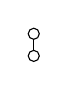
\begin{tikzpicture}
\draw (0pt,2pt) -- (0pt,6pt);
\draw (0pt,0pt) circle (2pt);
\draw (0pt,8pt) circle (2pt);
\end{tikzpicture}
} 

\newcommand{\dB}{
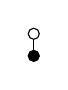
\begin{tikzpicture}
\draw (0pt,2pt) -- (0pt,6pt);
\draw[fill] (0pt,0pt) circle (2pt);
\draw (0pt,8pt) circle (2pt);
\end{tikzpicture}
} 

\newcommand{\dAA}{
\begin{tikzpicture}
\draw (0pt,0pt) -- (0pt,8pt);
\draw (0pt,0pt) -- (8pt,0pt);
\draw (8pt,8pt) -- (0pt,8pt);
\draw (8pt,8pt) -- (8pt,0pt);
\end{tikzpicture}
} 

\newcommand{\dBB}{

\begin{tikzpicture}
\draw[line width=1.5pt] (0pt,0pt) -- (0pt,8pt);
\draw[line width=1.5pt] (0pt,0pt) -- (8pt,0pt);
\draw (8pt,8pt) -- (0pt,8pt);
\draw (8pt,8pt) -- (8pt,0pt);
\end{tikzpicture}
} 
%-------------------------------------------------------------------------------
% Large draw commands
\newcommand{\dheA}
{
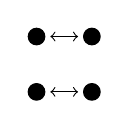
\begin{tikzpicture}
\draw [<->] (5pt, 0pt) -- (15pt, 0pt);
\draw [<->] (5pt, 20pt) -- (15pt, 20pt);
\draw[fill] (0pt,0pt) circle (3pt);
\draw[fill] (0pt, 20pt) circle (3pt);
\draw[fill] (20pt, 0pt) circle (3pt);
\draw[fill] (20pt, 20pt) circle (3pt);
\end{tikzpicture}
}

\newcommand{\dheB}
{
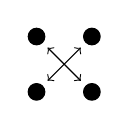
\begin{tikzpicture}
\draw [<->] (4pt, 4pt) -- (16pt, 16pt);
\draw [<->] (4pt, 16pt) -- (16pt, 4pt);
\draw[fill] (0pt,0pt) circle (3pt);
\draw[fill] (0pt, 20pt) circle (3pt);
\draw[fill] (20pt, 0pt) circle (3pt);
\draw[fill] (20pt, 20pt) circle (3pt);
\end{tikzpicture}
}

\newcommand{\dhoA}{
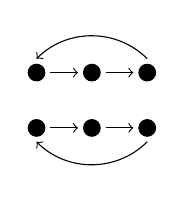
\begin{tikzpicture}
\draw [->] (5pt, 0pt) -- (15pt, 0pt);
\draw [->] (5pt, 20pt) -- (15pt, 20pt);
\draw [->] (25pt, 0pt) -- (35pt, 0pt);
\draw [->] (25pt, 20pt) -- (35pt, 20pt);
\draw [->] (40pt, -5pt) to [out=-135,in=-45] (0pt, -5pt);
\draw [->] (40pt, 25pt) to [out=135,in=45] (0pt, 25pt);
 
\draw[fill] (0pt,0pt) circle (3pt);
\draw[fill] (0pt, 20pt) circle (3pt);
\draw[fill] (20pt, 0pt) circle (3pt);
\draw[fill] (20pt, 20pt) circle (3pt);
\draw[fill] (40pt, 0pt) circle (3pt);
\draw[fill] (40pt, 20pt) circle (3pt);
\end{tikzpicture}
}

\newcommand{\dhoB}{
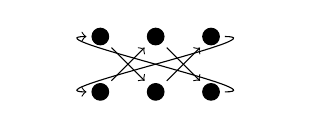
\begin{tikzpicture}
\draw [->] (4pt, 4pt) -- (16pt, 16pt);
\draw [->] (4pt, 16pt) -- (16pt, 4pt);
\draw [->] (24pt, 4pt) -- (36pt, 16pt);
\draw [->] (24pt, 16pt) -- (36pt, 4pt);
\draw [->] (45pt, 20pt) to [out=0,in=180] (-5pt, 0pt);
\draw [->] (45pt, 0pt) to [out=0,in=180] (-5pt, 20pt);
 
\draw[fill] (0pt,0pt) circle (3pt);
\draw[fill] (0pt, 20pt) circle (3pt);
\draw[fill] (20pt, 0pt) circle (3pt);
\draw[fill] (20pt, 20pt) circle (3pt);
\draw[fill] (40pt, 0pt) circle (3pt);
\draw[fill] (40pt, 20pt) circle (3pt);
\end{tikzpicture}
}